% Florian Sihler, 2026
% Licensed under the LPPL 1.3c, https://www.latex-project.org/lppl.txt
% All data here is made up.
\documentclass[a4paper]{article}
\usepackage[margin=1.5cm]{geometry}
\usepackage[T1]{fontenc}
\usepackage{siunitx}
\usepackage{tikz-sankey}
\usetikzlibrary{patterns}
\pagestyle{empty}
\setlength\parindent{0pt}
\begin{document}\sffamily

% the week of a cat, in hours
\begin{sankeypicture}[siunitx, column sep=auto, height=60mm, min pitch=4mm, value suffix={\,h},
   label={\sankeyName\enspace\textcolor{black!50}{\sankeyValue}}, column titles={week, mood, activity}]
   \sankeyNodes[color=black!35]{week = {one week}}
   \sankeyNodes[color=sankey-1]{lazy = lazy, sleep = sleeping, loaf = loafing in the sun}
   \sankeyNodes[color=sankey-2]{busy = busy, judge = judging humans, knock = knocking things off tables,
      zoom = zoomies at 3\,am}
   \sankeyNodes[color=sankey-3]{hungry = hungry, food = eating, beg = begging for food}
   \sankeyFlows{
      week -> lazy : 118,
      week -> busy : 31,
      week -> hungry : 19,
      lazy -> sleep : 96,
      lazy -> loaf : 22,
      busy -> judge : 17,
      busy -> knock : 9,
      busy -> zoom : 5,
      hungry -> food : 7,
      hungry -> beg : 12
   }
\end{sankeypicture}

\bigskip
% where the socks of a year went: every pair (washing, place) has a count
\begin{sankeypicture}[height=40mm, column sep=auto, flow opacity=.55, flow tint=100, node sep=1mm,
   column titles={washed in, ended up in}, percent precision=0,
   label={\sankeyName\enspace\textcolor{black!50}{\sankeyShare}},
   palette={sankey-5, sankey-1, sankey-6, sankey-4, sankey-3, black!45}]
   \foreach \m/\i in {cold wash/1, hot wash/2, by hand/3}{
      \foreach \p/\j in {the drawer/1, behind the dryer/2, the dog/3, another dimension/4}{
         \pgfmathtruncatemacro\n{mod(5*\i+7*\j,13)+2}
         \sankeyFlow{\m}{\p}{\n}}}
\end{sankeypicture}

\newpage
% alluvia: who wants which pizza
\begin{sankeypicture}[alluvial, unit=.5mm, column sep=32mm, column titles={age, topping, verdict},
   group colors={pineapple=sankey-2, no pineapple=sankey-5}]
   \sankeyFlows{
      kids -> cheese -> delicious : 30 [group=no pineapple],
      kids -> hawaii -> delicious : 12 [group=pineapple],
      kids -> hawaii -> a crime : 4 [group=pineapple],
      teens -> salami -> delicious : 22 [group=no pineapple],
      teens -> hawaii -> a crime : 15 [group=pineapple],
      adults -> salami -> a crime : 6 [group=no pineapple],
      adults -> cheese -> delicious : 18 [group=no pineapple],
      adults -> hawaii -> delicious : 9 [group=pineapple],
      grandmas -> cheese -> delicious : 10 [group=no pineapple],
      grandmas -> hawaii -> delicious : 7 [group=pineapple]
   }
\end{sankeypicture}

\bigskip
% routes: a coffee budget, steered by hand
\definecolor{bean}{HTML}{6F4E37}
\definecolor{crema}{HTML}{D9A066}
\definecolor{spill}{HTML}{C0392B}
\begin{tikzpicture}
   \sankeySetup{unit=.6mm, route radius=2.5mm, siunitx, value suffix={\,\texteuro},
      every route label/.style={font=\scriptsize, align=center},
      every bar/.style={postaction={pattern=crosshatch dots, pattern color=white}}}
   % the money comes in from the left and fades in
   \sankeyStart[angle=0, color=bean]{budget}{60}
   \sankeyRoute{budget}{label side=behind, label={pocket money\\\sankeyValue}, fade=in, forward=14mm, bar=2mm,
      label side=north, label={coffee budget}}
   \sankeySplit{budget}{beans=14, cafe=34, spilled=12}
   \sankeyRoute{beans}{color=crema, forward=12mm, left=90, fade=out, forward=10mm, label={beans\\\sankeyValue}}
   \sankeyRoute{spilled}{color=spill, forward=3mm, right=90, forward=4mm, arrow=2mm, label={spilled\\\sankeyValue}}
   \sankeyRoute{cafe}{forward=20mm, bar=2mm}
   \sankeySplit{cafe}{latte=20, cake=14}
   \sankeyRoute{latte}{forward=6mm, left=40, right=40, fade=out, forward=12mm, label={oat latte\\\sankeyValue}}
   \sankeyRoute{cake}{color=crema, forward=3mm, right=40, left=40, fade=out, forward=15mm,
      label={cake, by accident\\\sankeyValue}}
\end{tikzpicture}
\hfill
% top to bottom, as Mermaid writes it
\begin{sankeymermaid}[direction=down, height=45mm, column sep=14mm, flow fade=in]
---
config:
  sankey:
    showValues: false
    linkColor: source
---
sankey-beta
%% where the leftovers of a party go
Pizza,Fridge,6
Pizza,Breakfast,4
Cake,Fridge,3
Cake,Neighbour,2
Fridge,Breakfast,5
Fridge,Bin,4
\end{sankeymermaid}

\bigskip
% buckets: every stage of a pipeline is a bar of slots, and work moves from slot to slot
\begin{sankeypicture}[bucket bars, height=50mm, width=\linewidth, bucket count=10]
   \sankeyColumn[buckets=6]{import}
   \sankeyFlows{
      import@1 -> clean@2 : 1,
      import@2 -> clean@2 : .7,
      import@3 -> import@5 : .5,
      clean@2 -> model@5 : 1,
      clean@4 -> model@3 : .6,
      clean@7 -> plot@9 : .8,
      model@6 -> model@2 : .4,
      model@3 -> plot@4 : .6
   }
\end{sankeypicture}
\end{document}
